\documentclass[10pt,letterpaper]{article}

\usepackage[margin=0.75in]{geometry}
\usepackage{tikz}
\usepackage{graphicx}
\graphicspath{{images/}}
\begin{document}

  \title{Stats 314, Data Analysis \#1}
  \author{Cody Malick\\
  \texttt{malickc@oregonstate.edu}}
  \date{\today}
  \maketitle

\section*{Part I}
\subsection*{a}
Uniform distribution, because it is continuous, each time has an equal
probability, and distribution. This is a property unique to uniform
distributions.

\subsection*{b}
Poisson distribution, because we are given an average rate over a discrete
random variable. 

\subsection*{c}
Exponentional distribution, we're given a continuous random variable with an
average rate $(8)$, while also being given a skew indicating an exponential
distribution.

\subsection*{d}
Binomial distribution, as we are given a set of independent events, two 
possible outcomes, a probability of failure $(.25)$ and through that success
$(.75)$. 

\subsection*{e}
Normal distribution, as we are given an average value $(6)$, the standard
deviation from that value $(.6)$, and are told that values farther from the
median value are less likely. This describes a typical bell curve. 

\section*{Part II}
\subsection*{a}
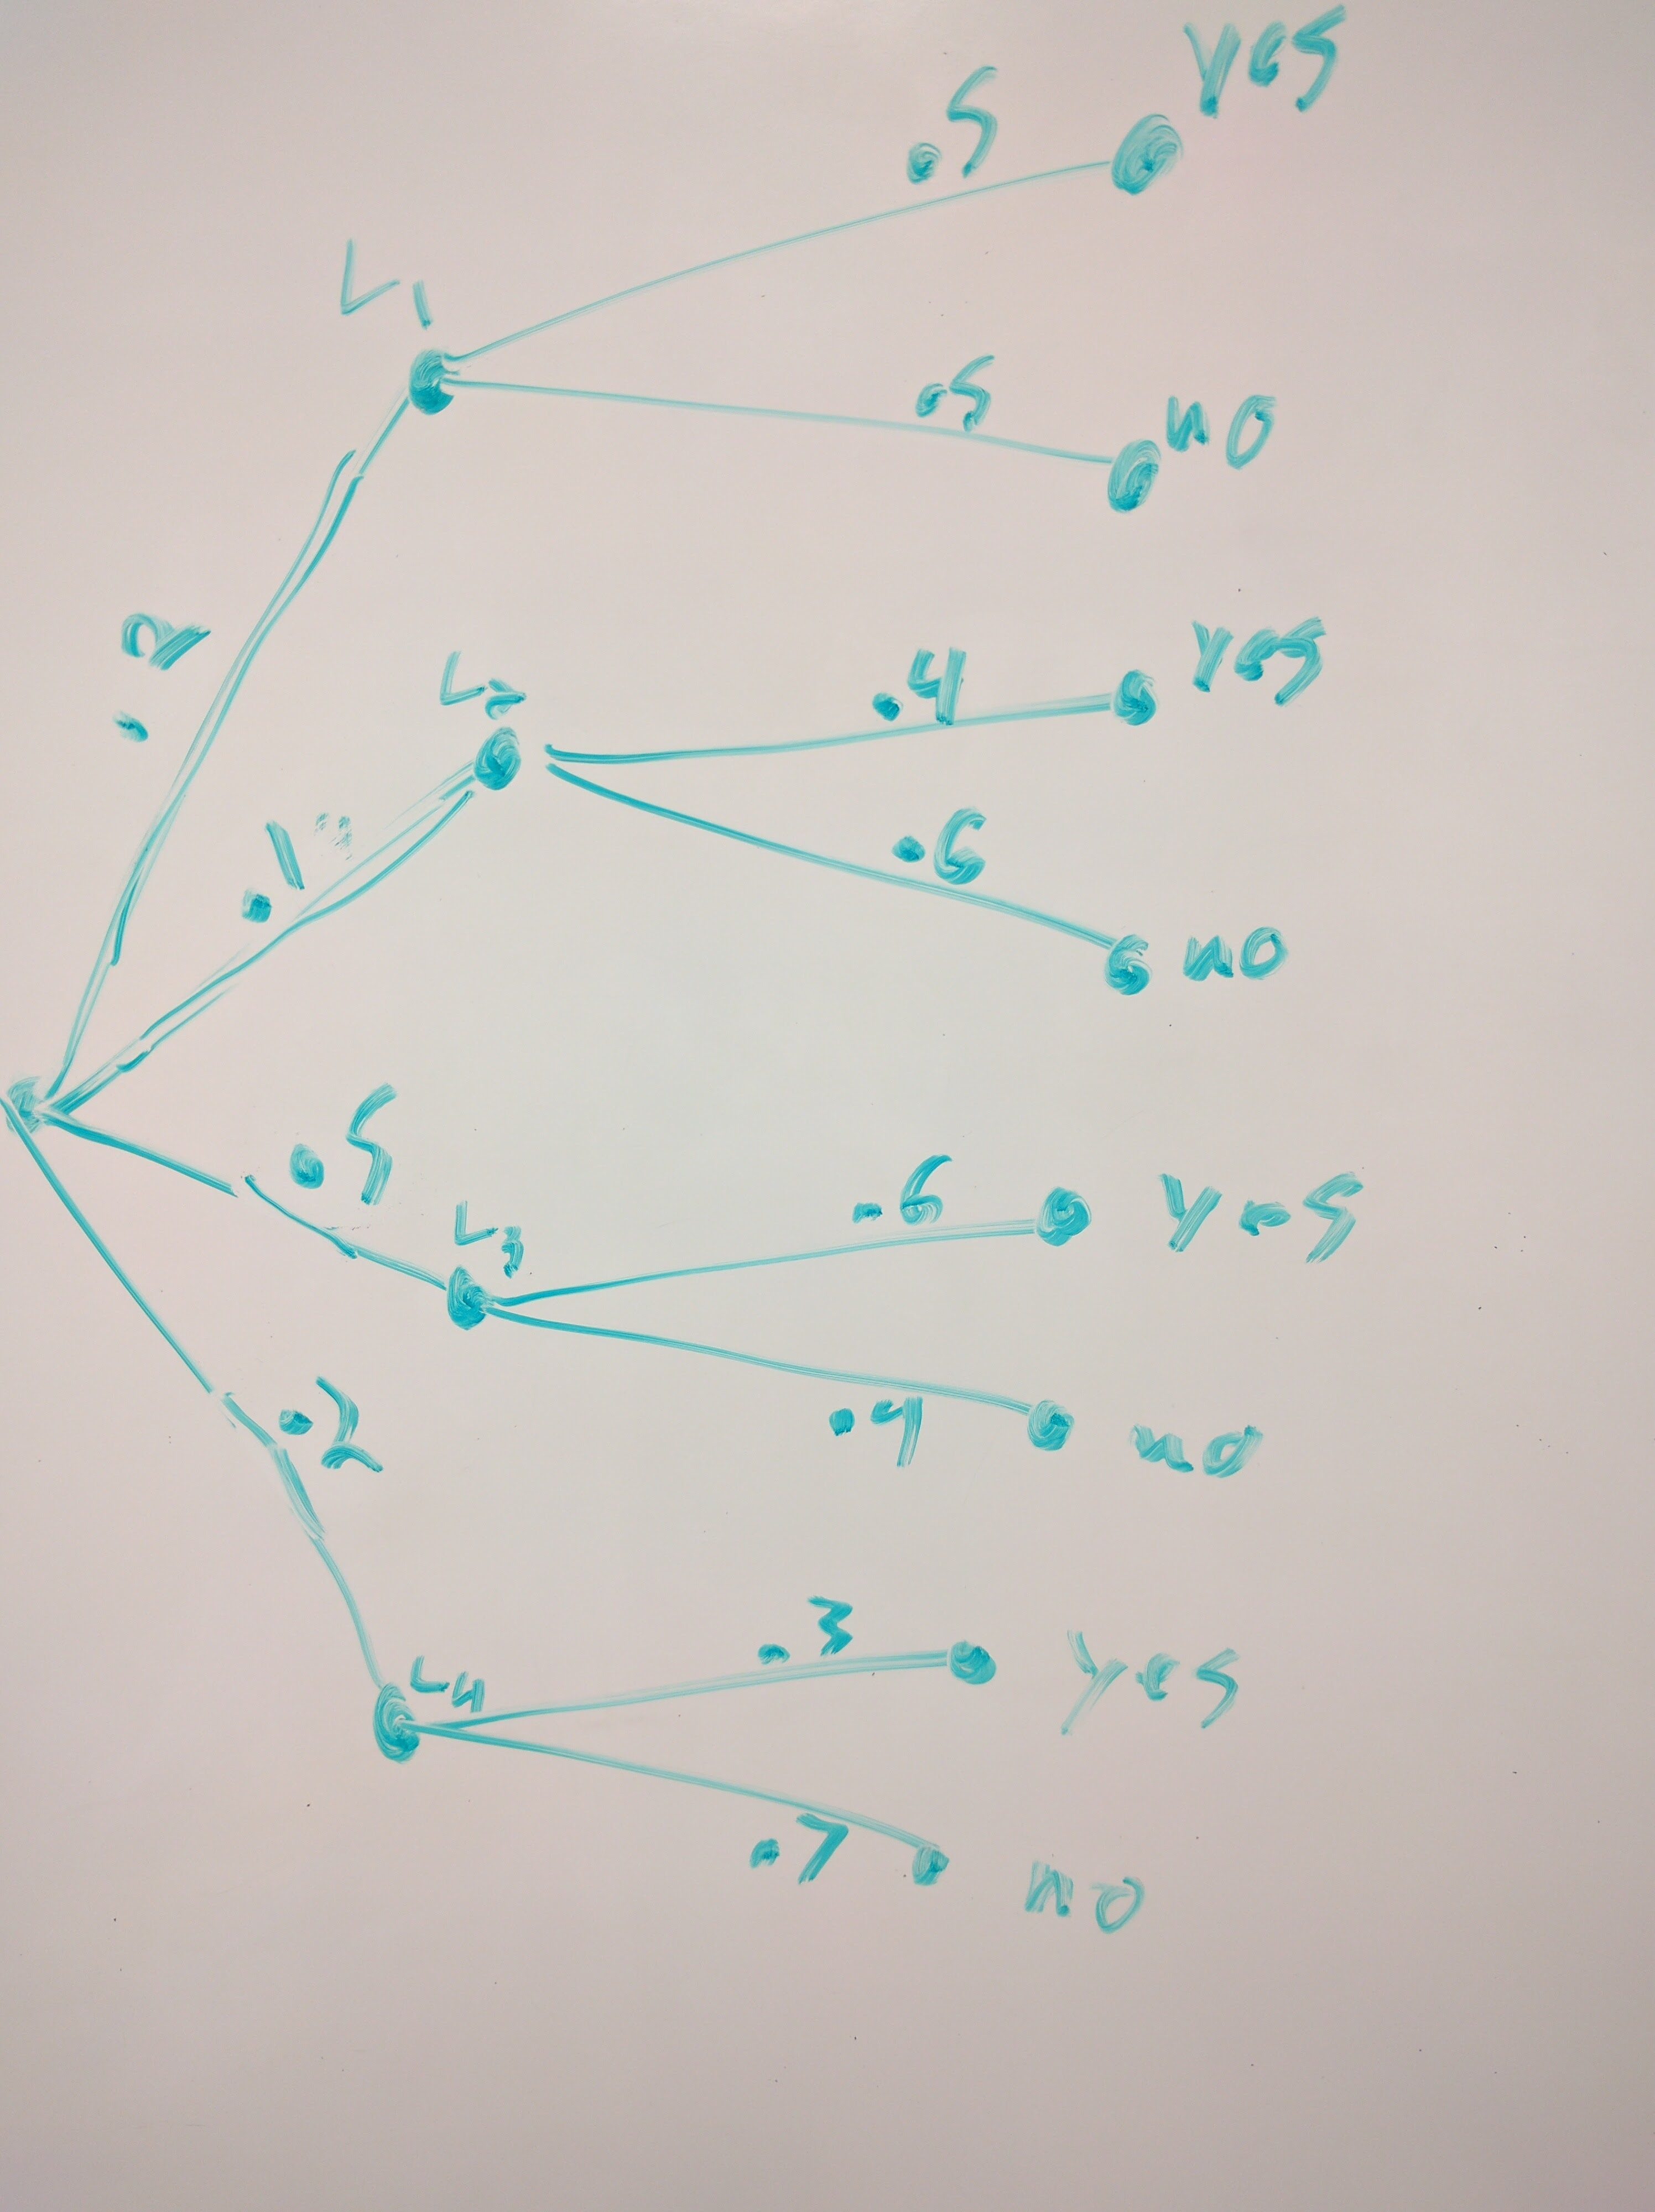
\includegraphics[scale=.1]{tree}

\subsection*{b}
To get the probability of a ticket, we have to use the law of total probability
to calculate the combined probability of getting a ticket in each area given
that they are in operation.

\noindent L1: $ .2*.5=.1 $\\
L2: $ .1*.4=.04 $\\
L3: $ .5*.6=.3 $\\
L4: $ .2*.3=.06 $\\
\\
P(ticket)=$ .1+.04+.3+.06=.5$

\section*{Part III}
\subsection*{a}
HHHH\\
HHHT\\
HHTH\\
HTHH\\
THHH\\
HHTT\\
HTHT\\
THHT\\
THTH\\
HTTH\\
TTHH\\
HTTT\\
THTT\\
TTHT\\
TTTH\\
TTTT\\
\subsection*{b}
$4/16=.25$
\subsection*{c}
$5/16=.3125$
\subsection*{d}
Binomial distribution, because we have a set of independent events with a discrete
random variable, and we're interested in the success rate for specific outcomes.
\subsection*{e}
To get the probability of $X = 3$, we have to take:\\
$P(X=3) = 4/16 = .25$
\subsection*{f}
To get the probability of $X >= 3$, we have to take:\\
$1-P(X>=3) = 1-(P(0)+P(1)+P(2)) = 1-.6875 = .3125$
\subsection*{g}
They sure are!
\subsection*{h}
The most likely number is 2. The likelihood is .375\\
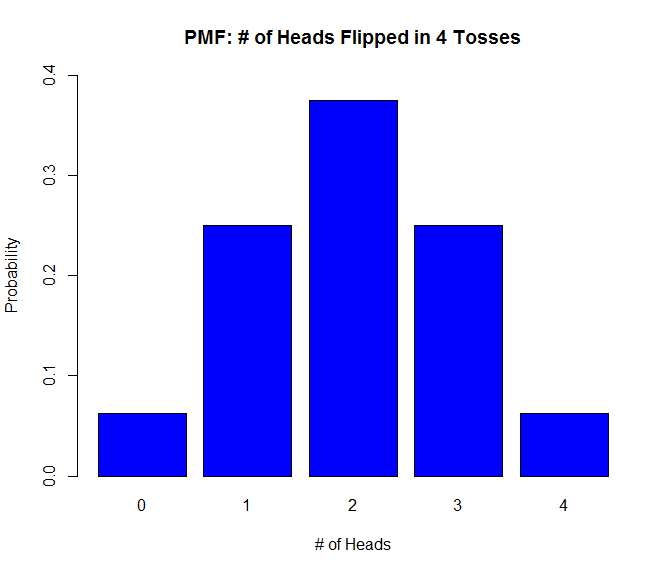
\includegraphics[scale=.75]{CoinPMF}

\subsection*{i}
$E(X)=np$, where $n$ is the number of coin tosses, and $p$ is the probability
of success.\\
$E(X)=4*.5=2$, which is our most likely number of heads/tails.

\section*{Part IV}

\section*{Part V}

\end{document}
